\documentclass{article}

\usepackage[dutch]{babel}
\usepackage[margin=3cm]{geometry}
\usepackage{graphicx}

\graphicspath{
    {img/}
}

\newcommand{\bold}[1]{\textbf{#1}}

\begin{document}

\begin{titlepage}
    \author{Tuur Vanhoutte}
    \title{Sensors \& Interfacing}
\end{titlepage}

\pagenumbering{gobble}
\maketitle
\newpage
\tableofcontents
\newpage

\pagenumbering{arabic}

\section {Communicatie}
\subsection{Datacommunicatie in IoT}
3 lagen:
\begin{enumerate}
    \item Application Layer
    \item Fog layer
    \item IoT Device Layer
\end{enumerate}

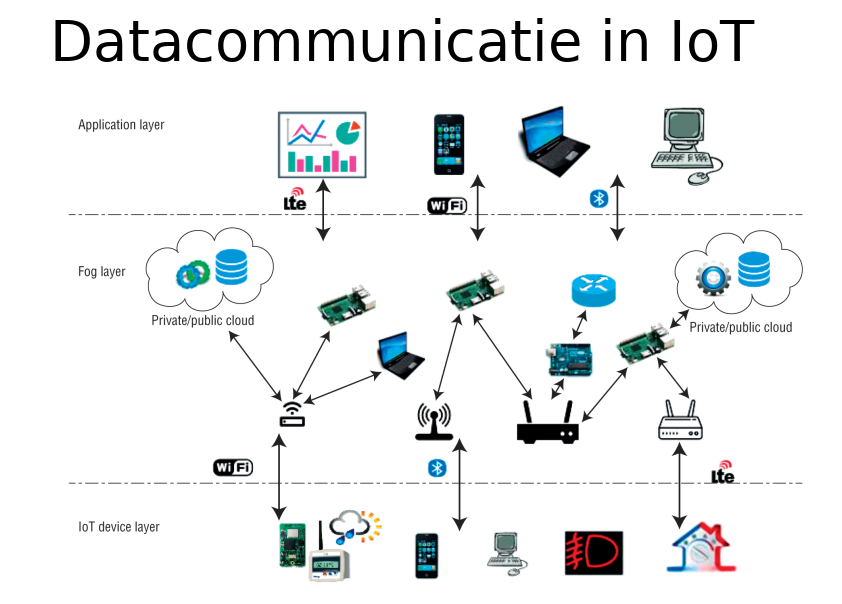
\includegraphics[width=1\textwidth]{Screenshot_20200210_120010.png}

\subsection{Data}
\begin{itemize}
    \item "Pre-informatie"
    \item Gegevens waaruit informatie kan worden gewonnen
    \item Stelt een bepaalde toestand voor
\end{itemize}

\subsection{Communicatie}
Overbrengen van informatie tussen deelnemers
\begin{itemize}
    \item Boodschap
    \item Signaal
    \item Medium
\end{itemize}

\subsubsection{Communicatieafspraken}
\begin{itemize}
    \item Coderen van informatie (encoding)
    \item Voorbeeld:
        \item morse-code
        \item Ascii-codering
        \begin{itemize}
            \item 
        \end{itemize}
        \item ...
\end{itemize}

\end{document}
